\begin{frame}
    \frametitle{Customizable Contraction Hierarchies}
    \begin{itemize}
        \item CH insert shortcut if shortest path property is violated
        \item CCH insert shortcut if there is no direct connection
    \end{itemize}
    \vfill
    \centering
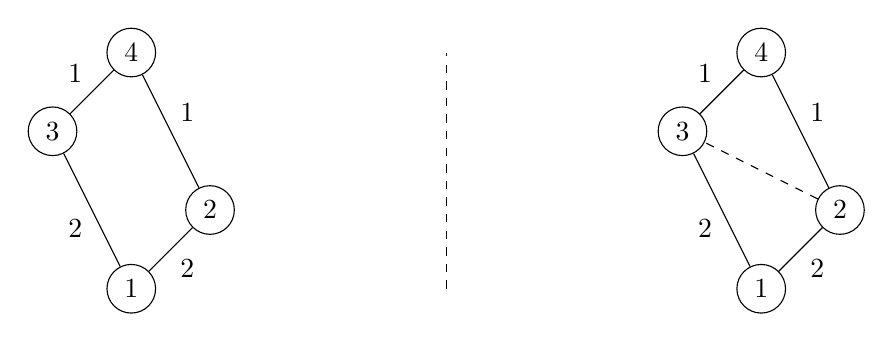
\begin{tikzpicture}[node distance={15mm}, main/.style = {draw, circle}]

    \node[main] (x3) at (0, 2) {$3$};
    \node[main] (x4) at (1, 3) {$4$};
    \node[main] (x2) at (2, 1) {$2$};
    \node[main] (x1) at (1, 0) {$1$};
    
    \draw (x1) -- node[below right] {$2$}(x2);
    \draw (x1) -- node[below left] {$2$} (x3);
    \draw (x2) -- node[above right] {$1$} (x4);
    \draw (x3) -- node[above left] {$1$} (x4);

    \draw[dashed]  (5,0) -- (5,3);

    \node[main] (x31) at (8, 2) {$3$};
    \node[main] (x41) at (9, 3) {$4$};
    \node[main] (x21) at (10, 1) {$2$};
    \node[main] (x11) at (9, 0) {$1$};
    
    \draw (x11) -- node[below right] {$2$}(x21);
    \draw (x11) -- node[below left] {$2$} (x31);
    \draw (x21) -- node[above right] {$1$} (x41);
    \draw (x31) -- node[above left] {$1$} (x41);
    \draw[dashed] (x21) -- node[above, sloped] {}  (x31);

    
\end{tikzpicture}
\end{frame}